\documentclass[11pt]{article}
\usepackage[a4paper,margin=22mm,headheight=16pt]{geometry}
\usepackage{fontspec,xeCJK,xcolor,graphicx,enumitem,fancyhdr,titlesec}
\usepackage{hyperref}
\IfFontExistsTF{Times New Roman}{\setmainfont{Times New Roman}}{\setmainfont{TeX Gyre Termes}}
\IfFontExistsTF{FangSong}{\setCJKmainfont[AutoFakeBold=2]{FangSong}}{\IfFontExistsTF{仿宋}{\setCJKmainfont[AutoFakeBold=2]{仿宋}}{\IfFontExistsTF{FandolFang-Regular.otf}{\setCJKmainfont[AutoFakeBold=2]{FandolFang-Regular.otf}}{\setCJKmainfont{FandolSong-Regular.otf}}}}
\definecolor{ink}{HTML}{173747}\definecolor{accent}{HTML}{227E82}
\hypersetup{colorlinks=true,urlcolor=accent,linkcolor=accent}
\linespread{1.22}\setlength{\parindent}{0pt}\setlength{\parskip}{6pt}
\setlist[itemize]{leftmargin=1.4em,itemsep=3pt}
\titleformat{\section}{\large\bfseries\color{ink}}{}{0pt}{}
\titlespacing*{\section}{0pt}{14pt}{7pt}
\pagestyle{fancy}\fancyhf{}\lhead{\small OMNI LEARNING / Learning guide}\rhead{\small Source-grounded learning}\cfoot{\small\thepage}
\emergencystretch=2em\widowpenalty=10000\clubpenalty=10000
\newcommand{\Needspace}[1]{\par\begingroup\dimen0=#1\relax\vskip0pt plus\dimen0\penalty-100\vskip0pt plus-\dimen0\vskip\dimen0\penalty9999\vskip-\dimen0\vskip0pt\endgroup}
\begin{document}


{\LARGE\bfseries\color{ink} Stars or Planets? Read the Sky with a Phone Chart}\par

2026-10-09 | Day01/3 | Read 10 min + practice 5 min\par\vspace{6pt}

\Needspace{5\baselineskip}\section*{Today's goal and a 2-minute starting question}

By the end, you will be able to check whether a bright point is a star or a planet using its position and a phone chart, and explain why twinkling alone cannot settle the question. You need no telescope. [S2]

Before reading, write your first answer: A steady bright point must be a planet: true or false, and why? Keep it for the self-check. Allow 10 minutes for this question, reading and figure study, then 5 minutes for practice and answers. This is an estimate; outdoor observing is optional.

\Needspace{5\baselineskip}\section*{1. Describe where to look}

Treat the sky as a dome. Your horizon is the zero-height reference; directly overhead is the zenith. A chart's altitude means angular height above that horizon, not an object's distance from Earth: 0 degrees is on the horizon, 90 degrees is overhead, and a negative altitude is below it. A building can block a point even when its altitude is positive. [S4]

Direction answers which way?; altitude answers how high? You can start with north, east, south and west. If a chart gives azimuth measured from north toward east, 90 degrees means east and 180 degrees means south. Check its convention. [S4]

Study the Day1 panel below: the traveler compares a point and its surrounding pattern with a chart. The drawing cannot name that point; its pattern is invented. The useful action is matching positions after checking settings. The other panels only mark later topics.

\begin{center}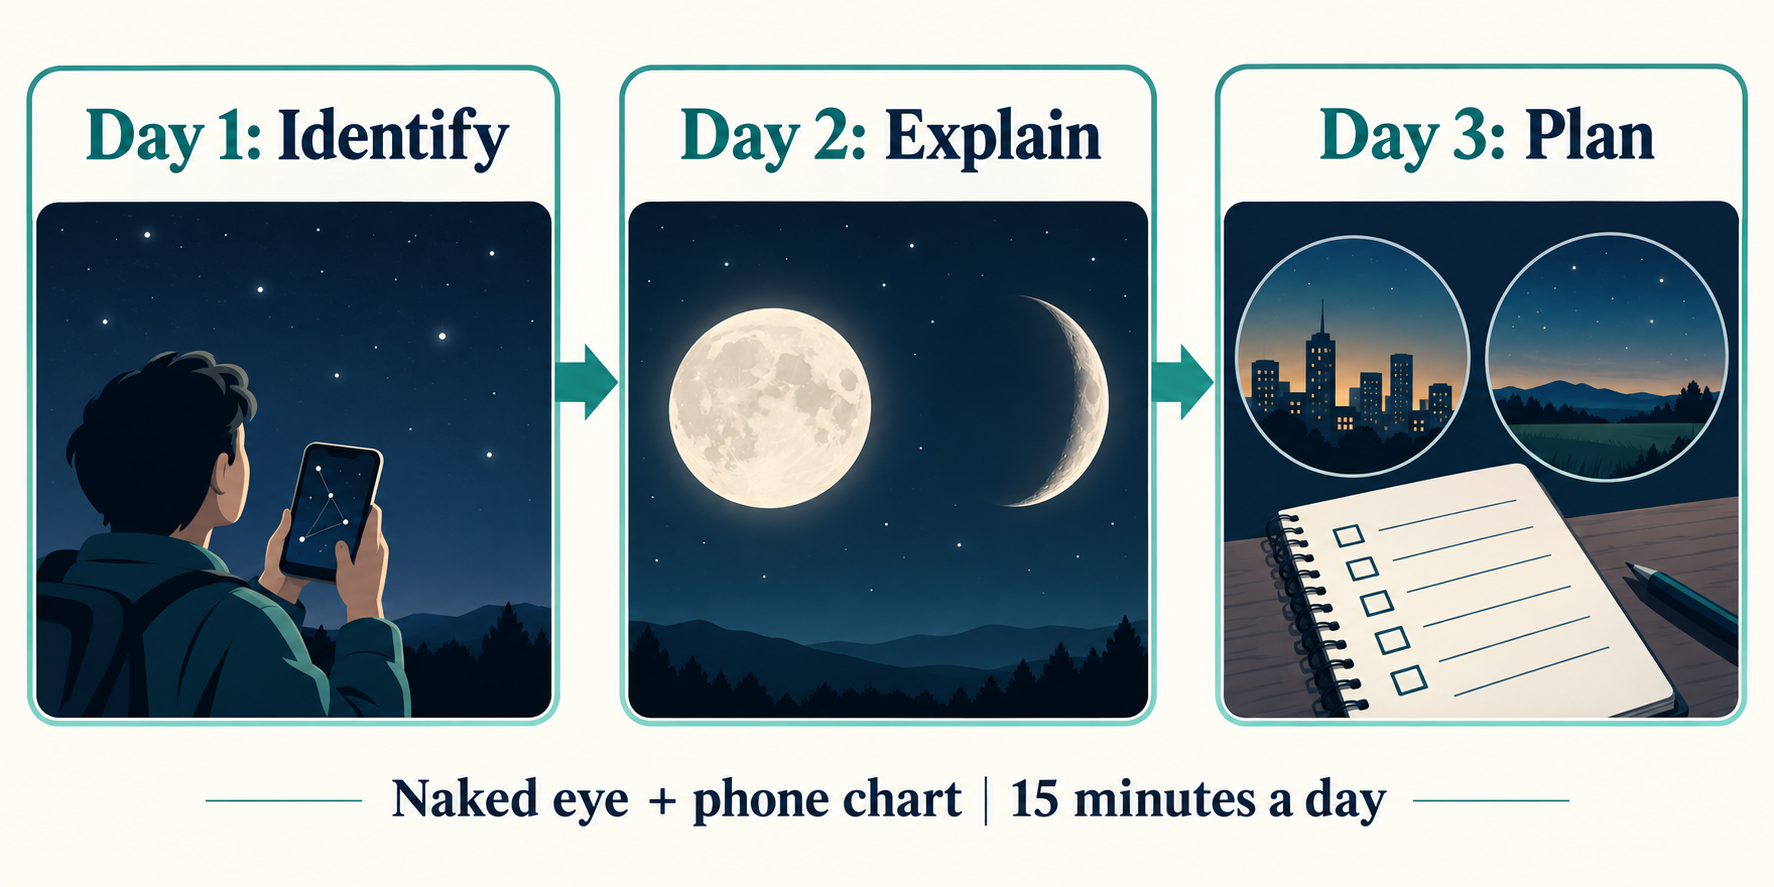
\includegraphics[width=\linewidth,height=0.26\textheight,keepaspectratio]{../assets/figure-8540a079e446.png}\par

{\small Study the Day1 panel: compare position and pattern with a correctly set chart. It cannot identify the drawn point. Later panels are course navigation; Moon icons are alternative appearances.}\par

{\footnotesize AI-generated teaching illustration reused from this course’s reviewed plan. Invented sky pattern; no observation or official diagram. Original prompt and provenance retained in research/.}\end{center}

\Needspace{5\baselineskip}\section*{2. Know what the clues can tell you}

Stars supply their own light. The visible light we see from the planets in our solar system is mainly reflected sunlight. Both can look like small bright points to unaided eyes, so shine alone does not reveal which kind of object you are seeing. [S6]

Moving pockets of air bend starlight by changing amounts. A distant star is effectively a point source to the eye, so those changes can make it flicker. A planet has a larger apparent disc, even when you cannot resolve it; the atmospheric effects across that disc tend to average out. This is why planets usually look steadier. Use that tendency as a clue, not a certificate of identity. [S1]

Mercury, Venus, Mars, Jupiter and Saturn are familiar naked-eye candidates, but not necessarily visible together. Their positions shift against background stars over time. A point traveling across a large part of the sky in minutes could instead be a satellite; regular flashing can suggest an aircraft. These clues invite another check. [S5]

\Needspace{5\baselineskip}\section*{3. Use a chart to test your guess}

First set the chart to your observing place, date and local time. Traveling can leave an old city selected; simulation mode can leave the wrong time selected. Those settings matter because direction and height change with place and time. [S3] [S4]

Select the point and read its name and category. Compare its direction, height and nearby pattern with what you see. Do not rely only on where the phone points: compass problems are possible. Use your app's calibration guidance if direction looks wrong. [S3]

An object displayed on a map is not automatically observable. Check below-horizon status, daylight and obstructions. City skyglow hides faint stars; rural darkness can make more points visible without changing their categories. [S2]

If the match fails, recheck settings and orientation, then leave the identification unresolved. That is a useful result. No phone app has been operated for this lesson; control names may differ in yours.

\Needspace{5\baselineskip}\section*{Worked example: a provisional identification}

This is invented practice data, not a sky prediction for China. Suppose a point appears roughly east, about one-third of the way from the horizon to overhead, and flickers. A correctly configured mock chart lists Object A: category star, east, altitude 30 degrees; Object B: category planet, west, altitude minus 5 degrees.

A is the plausible match because its direction and height fit. B cannot match this point: it is below the horizon and in a different direction. Flickering supports the guess but is not the decisive evidence. You would still compare nearby points and rule out a chart-orientation error before calling the identification confirmed.

Write: Probable star A; position agrees with the chart. I will verify the pattern. Do not write: Star, because it flickers.

\Needspace{5\baselineskip}\section*{5-minute practice: make two identification notes}

Minutes 1–3: indoors, open your existing chart. Confirm its location, date and displayed local time; this is rehearsal, not a prediction for a trip. Select one star and one planet. For each, record: name; category; direction; altitude or below-horizon status. Searching for an object does not mean it is currently visible.

If your chart is unavailable or controls take too long, use the mock records A and B above. Record their categories and positions, mark the location/date/time as hypothetical, not supplied, and explain why this dataset cannot establish real travel visibility.

Minute 4: answer your starting question again. Then explain why a planet drawn below the horizon cannot be the bright point above you.

Minute 5: compare with the answers below. Your output is two short records and one sentence explaining why a steady point still needs checking. Stop here; no field trip or expansion reading is required today.

\Needspace{5\baselineskip}\section*{Self-check answers and recap}

Starting question: false. A steady point is a candidate, not a confirmed planet; match its chart category and position using the right context.

Mock-record check: A is a star, east, altitude 30 degrees. B is a planet, west, altitude minus 5 degrees: below the horizon. These are teaching entries, not observations. The missing location/date/time prevents a real visibility claim.

For your own chart, categories and coordinates vary with the object and settings. A complete answer records the context, category and position; it need not find a planet above the horizon. If you omitted context, repeat that step rather than inventing a successful sighting.

Remember: describe the position, consider the clue, check the chart. Next lesson's question is why the Moon changes shape even though it also reflects sunlight. Day02 has not been generated. Optional links below are outside today's 15 minutes.

\Needspace{6\baselineskip}\section*{Further reading}\small Optional; outside the daily core time budget.\begin{enumerate}[leftmargin=1.6em]

\item [S1] \href{https://imagine.gsfc.nasa.gov/ask\_astro/night\_sky.html}{Why do stars twinkle while planets usually look steady?} — Find the answer by Koji Mukai and Maggie Masetti (question submitted 1998-12-17). Read the atmosphere and apparent-size explanation; ignore unrelated legacy links. Page updated 2020-10-22.\par NASA Goddard, Imagine the Universe! | Published: Not stated | Checked: 2026-10-09

\item [S2] \href{https://science.nasa.gov/skywatching/faq/}{Skywatching FAQ} — Read the tools and light-pollution answers. Connect naked-eye observing with realistic city expectations. Page last updated 2024-09-03.\par NASA Science | Published: Not stated | Checked: 2026-10-09

\item [S3] \href{https://www.timeanddate.com/astronomy/night/help}{How to Use the Night Sky Map} — Read object selection, date/time selection and compass troubleshooting. Compare these controls with your own chart; no new app is required.\par timeanddate.com | Published: Not stated | Checked: 2026-10-09

\item [S4] \href{https://www.timeanddate.com/astronomy/horizontal-coordinate-system.html}{Altitude and Azimuth: The Horizontal Coordinate System} — Read Altitude and Azimuth and Depends on Location and Time. Translate a chart position into direction and angular height.\par timeanddate.com; Konstantin Bikos | Published: Not stated | Checked: 2026-10-09

\item [S5] \href{https://science.nasa.gov/skywatching/}{Skywatching: What to Look for in the Sky} — Go to Planets and Satellites. Compare slow movement against background stars with a passing satellite; skip monthly event forecasts. Page last updated 2026-10-01.\par NASA Science | Published: Not stated | Checked: 2026-10-09

\item [S6] \href{https://science.gsfc.nasa.gov/attic/cosmicopia.gsfc.nasa.gov/qa\_study.html}{Cosmicopia: Studying and Exploring Space} — Find the stars-and-planets brightness answer dated June 2000. Use its own-light versus reflected-light distinction; unrelated archived guidance is outside this lesson.\par NASA Goddard; Dr. Eric Christian | Published: Not stated | Checked: 2026-10-09

\end{enumerate}

\end{document}